\documentclass[aspectratio=43]{beamer}
\usepackage{luatexja-fontspec}
\usepackage{graphicx,color,multicol,verbatim,listingsutf8}
\usepackage{xcolor}
\usepackage{url,tikz}
\usepackage[symbol]{footmisc}
\usetikzlibrary{arrows.meta,calc,fit,positioning}
\usetheme{Boadilla}
\usecolortheme[RGB={140,0,0}]{structure}
\setbeamertemplate{navigation symbols}{}
\setbeamercovered{transparent}
\usefonttheme{professionalfonts}
\renewcommand\familydefault{\rmdefault}
\renewcommand{\figurename}{図\thefigure}
\renewcommand{\thefootnote}{\fnsymbol{footnote}}
\setbeamertemplate{sections/subsections in toc}[sections numbered]
\setbeamertemplate{enumerate item}[default]
\setbeamertemplate{itemize item}[triangle]
\lstset{
        %枠外に行った時の自動改行
    breaklines = true,
        %自動改行後のインデント量(デフォルトでは20[pt])
    breakindent = 10pt,
        %標準の書体
    basicstyle = \ttfamily\small,
        %コメントの書体
    commentstyle = {\ttfamily \color[cmyk]{1,0.4,1,0}},
        %関数名等の色の設定
    classoffset = 0,
        %キーワード(int, ifなど)の書体
    keywordstyle = {\bfseries\ttfamily \color[cmyk]{0,1,0,0}},
        %表示する文字の書体
    stringstyle = {\ttfamily \color[rgb]{0,0,1}},
        %枠 tは上に線を記載, Tは上に二重線を記載
        %他オプション:leftline,topline,bottomline,lines,single,shadowbox
    frame = single,
        %frameまでの間隔(行番号とプログラムの間)
    framesep = 5pt,
        %行番号の位置
    numbers = left,
        %行番号の間隔
    stepnumber = 1,
        %行番号の書体
    numberstyle = \scriptsize,
        %タブの大きさ
    tabsize = 4,
        %キャプションの場所(tbならば上下両方に記載)
    captionpos = t,
    xleftmargin=1.5em
}
\makeatletter
\title{3. 音声合成}
\subtitle{情報学群実験第3c 3i}
\author{Group 10\thanks{門屋 陽丈\and 谷保 愛華\and 内藤 熙人\and 成岡 小雪\and 平林 里菜\and 三上 柊\and 溝口 洸熙}}
\date{2023.04.20}
\newcommand{\showsec}{\thesection .}
\setbeamercolor{block title}{bg=black,fg=white}
\setbeamercolor{block body}{bg=gray!10,fg=black}
\begin{document}
\begin{frame}
    \titlepage
\end{frame}
\begin{frame}
    \begin{multicols}{2}
        \tableofcontents
    \end{multicols}
\end{frame}
\section{初期位相・矩形波}
\begin{frame}[t]{\showsec 初期位相・矩形波}
    周波数\(f\),時刻を\(t\)に設定する.
    \begin{block}{初期位相}
        初期位相を\(\phi\)に設定する.
        \begin{align}
            y(t) & = \sin(2\pi ft+\phi)
        \end{align}
    \end{block}
    \begin{block}{短形波のフーリエ級数展開}
        \begin{align}
            y(t) & = \sum_{k=1}^{\infty}\dfrac{1}{2k-1}\sin\big(2\pi(2k-1)ft\big)
        \end{align}
    \end{block}
\end{frame}
\section{ノコギリ波}
\begin{frame}[t]{\showsec ノコギリ波}
    \begin{figure}
        \centering
        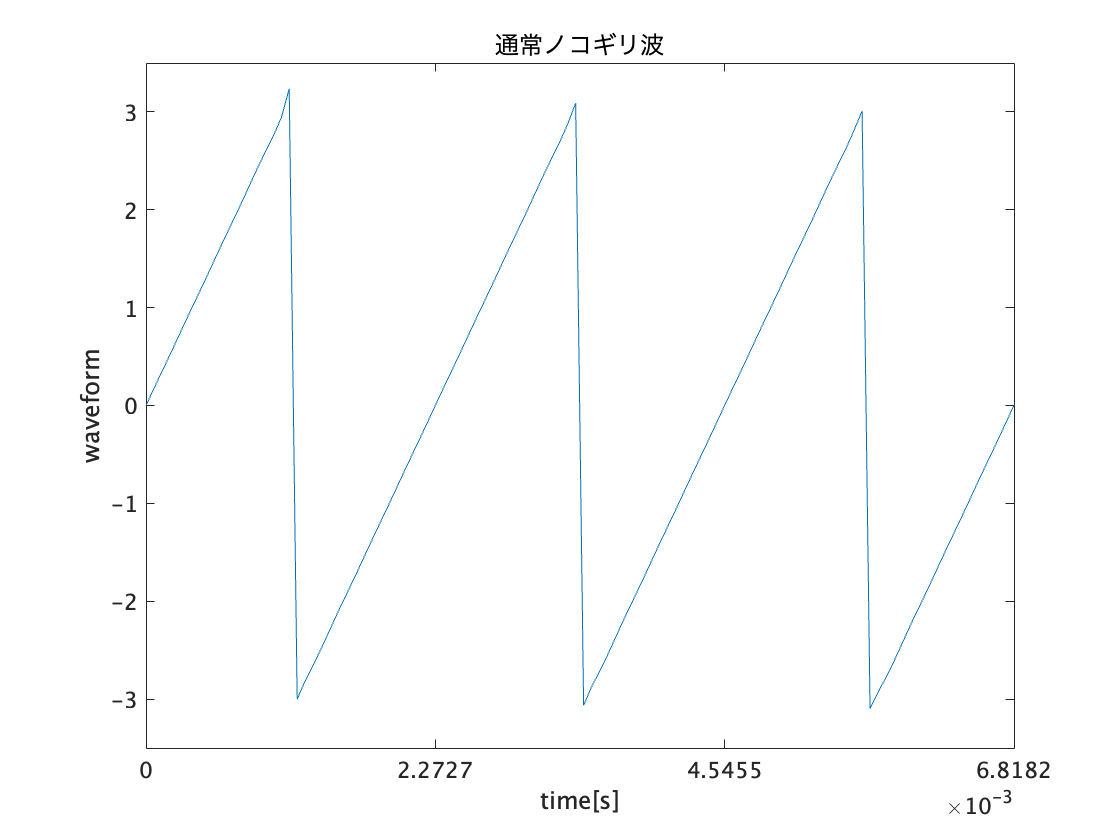
\includegraphics[keepaspectratio,width=0.85\textwidth]{nokogiri.png}
    \end{figure}
\end{frame}
\begin{frame}[t]{\showsec ノコギリ波}
    \begin{align}
        y(t) & =t             & (-\pi<t<\pi)     \\
        \intertext{を周期\(2\pi\)の関数として周期的に拡張したもの.}
        y(t) & = y(t + 2k\pi) & (k\in\mathbb{Z})
    \end{align}
    \begin{block}{ノコギリ波のフーリエ級数展開}
        \begin{align}
            y(t) & =\sum_{k=1}^{\infty}(-1)^{k-1}\dfrac{2}{k}\sin(kt)\label{nokogiri}
        \end{align}
    \end{block}
    \(\displaystyle\sum_{k=1}^{\infty}\)の\(\infty\)は今回,\texttt{50}としてプログラミングしている.
\end{frame}
\section{課題1}
\subsection{問題}
\begin{frame}[t,containsverbatim]{\showsec 課題1}
    \begin{exampleblock}{}
        矩形波,ノコギリ波を基本周波数 440Hz 等の可聴域の範囲で作成し,さらに各周波数成分も位相を適当な値に変化させよう.\\
        (サンプリング周波数\verb|Fs = 16kHz|,長さ\verb|2s|.)
        \begin{itemize}
            \item 位相の操作
                  \begin{itemize}
                      \item 固定値 \(\pi/4\)
                      \item 固定値 \(\pi/2\)
                      \item ランダム値\footnote{ランダム値は \texttt{variable = rand} で格納できる.}
                  \end{itemize}
        \end{itemize}
    \end{exampleblock}
    \begin{block}{Tips}
        \begin{lstlisting}[language={Matlab},numbers={none},frame={none},xleftmargin=0em]
axis([xmin xmax ymin ymax]);
        \end{lstlisting}
        グラフをプロットするときの範囲を指定できる.周波数\(f\)の周期関数を\texttt{n}周期分プロットしたい場合は\texttt{xmin}を\texttt{0},\texttt{xmax}を\texttt{n/f}に設定する.
    \end{block}
\end{frame}
\subsection{サンプルコード}
\begin{frame}[t,containsverbatim]{\showsec 課題1(サンプルコード)}
    \begin{lstlisting}[language={Matlab}]
clear all;
Fs = 16000; % サンプリング周波数
f = 400;    % 基本周波数
t = [0 : ??] /Fs % 時間軸テーブル
phi1 = pi / 4;   % 初期位相 pi/2
phi2 = pi / 2;   % 初期位相 pi/4
phi3 = rand;     % 初期位相 ランダム
% --- ノコギリ波生成 ---
for k=1:50 % とりあえず50にでも設定しておく
    y1 = ?? + (-1)^(k-1) * 1/3 * 2/k * sin(???);
    y2 = ...;
    y3 = ...;
end
...
\end{lstlisting}
\end{frame}
\subsection{結果:ノコギリ波}
\begin{frame}{\showsec 課題1(結果:ノコギリ波)}
    \begin{figure}
        \centering
        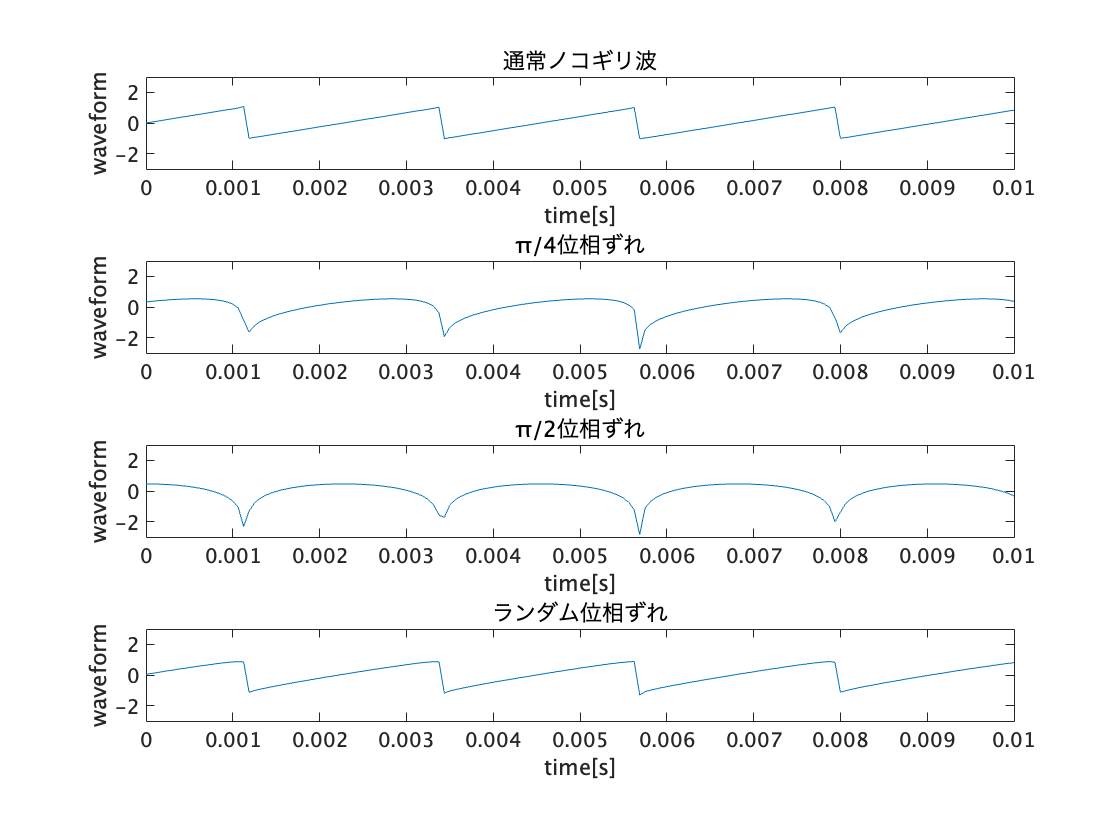
\includegraphics[keepaspectratio,width=0.89\textwidth]{no1_1_ans.png}
    \end{figure}
\end{frame}
\subsection{結果:矩形波}
\begin{frame}{\showsec 課題1(結果:矩形波)}
    \begin{figure}
        \centering
        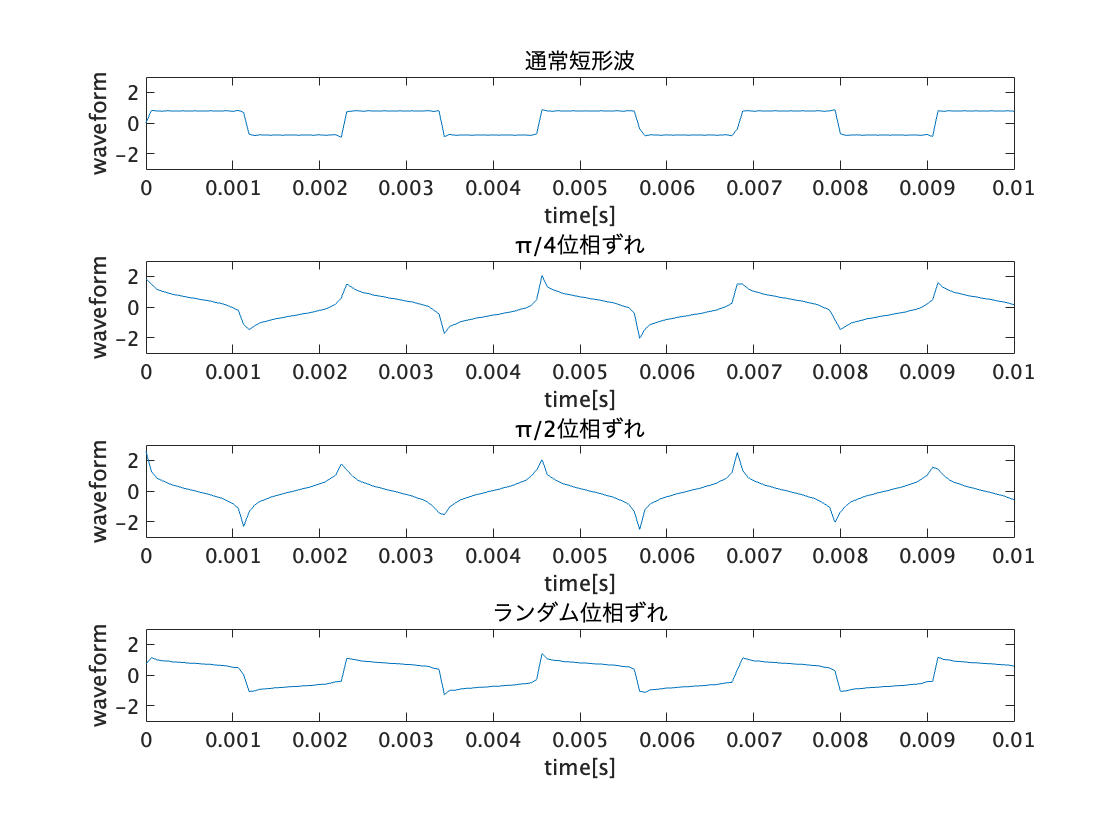
\includegraphics[keepaspectratio,width=0.89\textwidth]{no1_2_ans.png}
    \end{figure}
\end{frame}
\section{課題2}
\subsection{結果}
\begin{frame}[t]{\showsec 課題2}
    \begin{exampleblock}{}
        自分の母音の音声を4s程度ずつ録音し,その音声データの波形の上下を反転さよう.
        元データと反転後のデータを聴き比べよう.
    \end{exampleblock}
    \begin{figure}
        \centering
        \begin{minipage}[t]{0.49\textwidth}
            \centering
            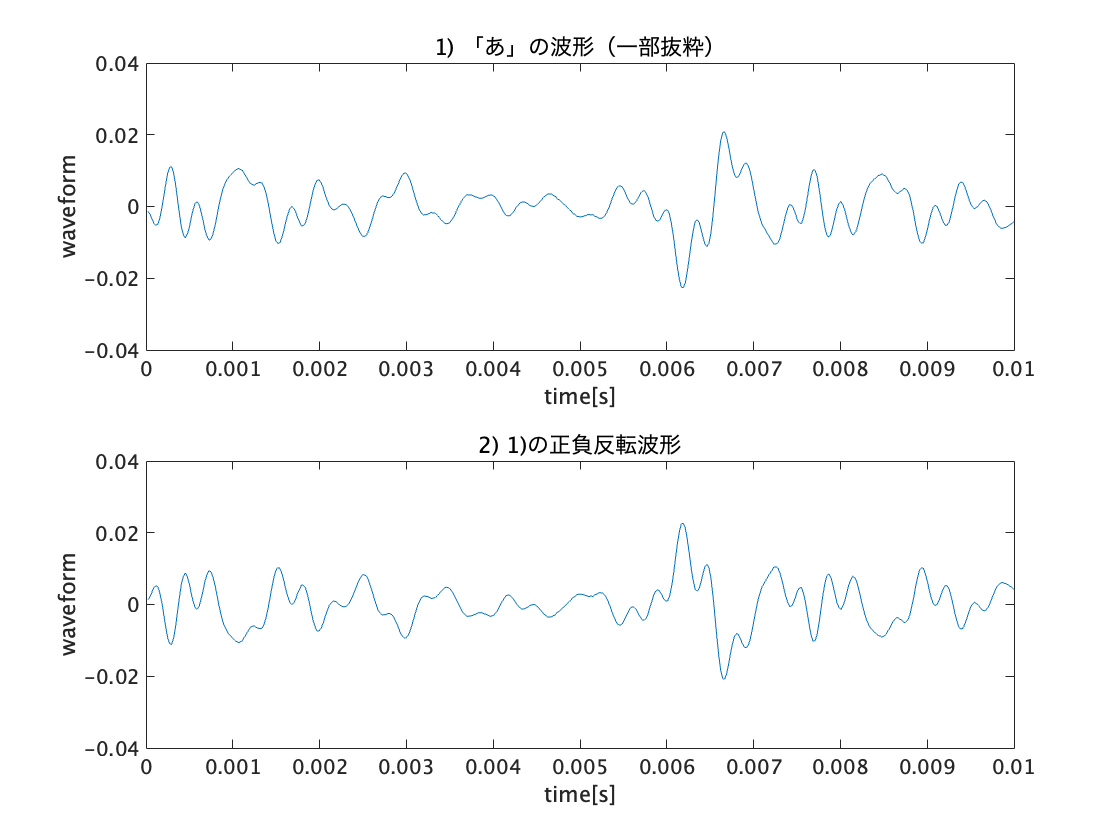
\includegraphics[keepaspectratio,width=\textwidth]{no2_ans_1.png}
            \caption{それぞれのグラフ}
        \end{minipage}
        \begin{minipage}[t]{0.49\textwidth}
            \centering
            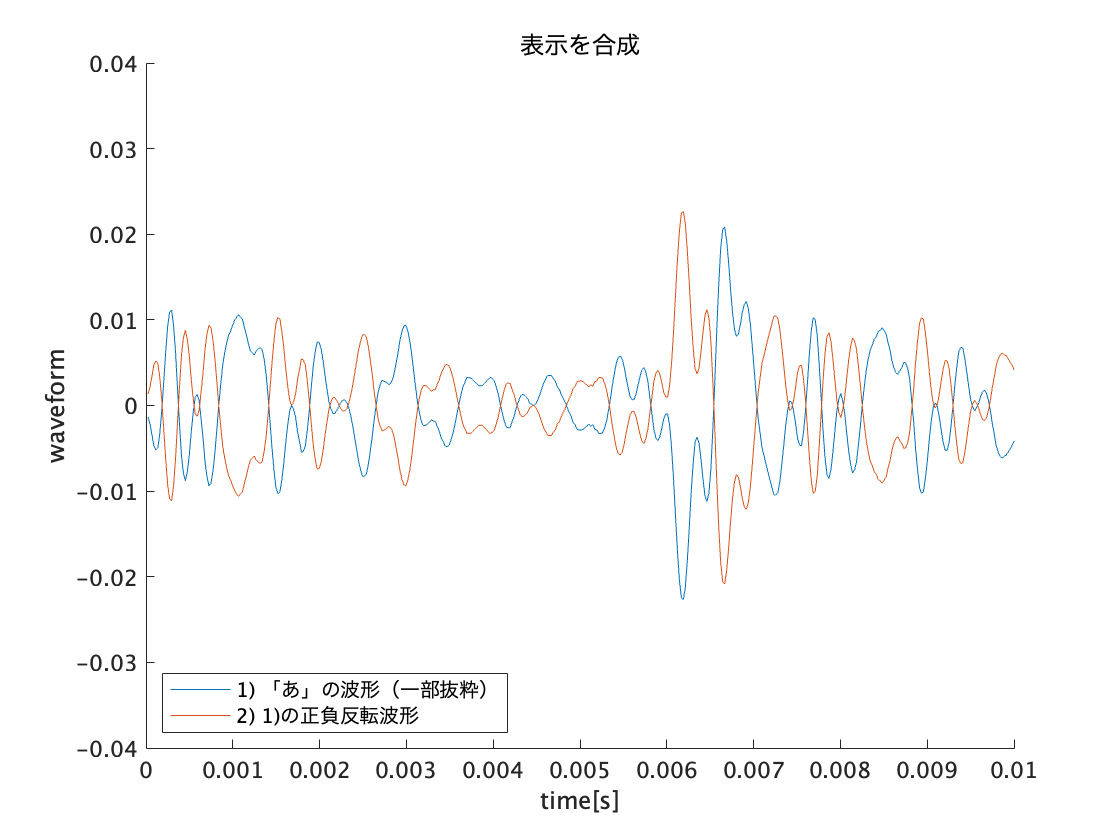
\includegraphics[keepaspectratio,width=\textwidth]{no2_ans_2.png}
            \caption{グラフを重ね合わせてみる}
        \end{minipage}
    \end{figure}
\end{frame}
\subsection{サンプルコード}
\begin{frame}[t,containsverbatim]{\showsec 課題2(サンプルコード)}
    \begin{lstlisting}[language={Matlab}]
clear;
[y, Fs] = audioread('sound1.wav');
y=?? % ステレオからモノラルへの変換
N = ??; % yの長さ
t = (1:??) /??; % 時間軸テーブル
z = ??; % yの各要素に対して正ならば負,負ならば正にする
...
    \end{lstlisting}
    \begin{alertblock}{}
        ステレオからモノラルへの変換をすること!
        \begin{itemize}
            \item さもなくば,左右それぞれの信号が処理されグラフが見難くくなる.
        \end{itemize}
    \end{alertblock}
\end{frame}
\addtocontents{toc}{\newpage}
\section{周波数解析}
\subsection{ノコギリ波}
\begin{frame}[t]{\showsec 周波数解析(ノコギリ波)}
    ノコギリ波は以下の式で表せる.
    \begin{align}
        y(t) & = \sum_{k=1}^{\infty}(-1)^{k-1}\dfrac{2}{k}\sin(kt)\tag{\ref{nokogiri}}    \\
             & = 2\sin(t) - \sin(2t) + \frac{2}{3}\sin(3t) - \frac{1}{2}\sin(4t) + \cdots
    \end{align}
    \begin{figure}
        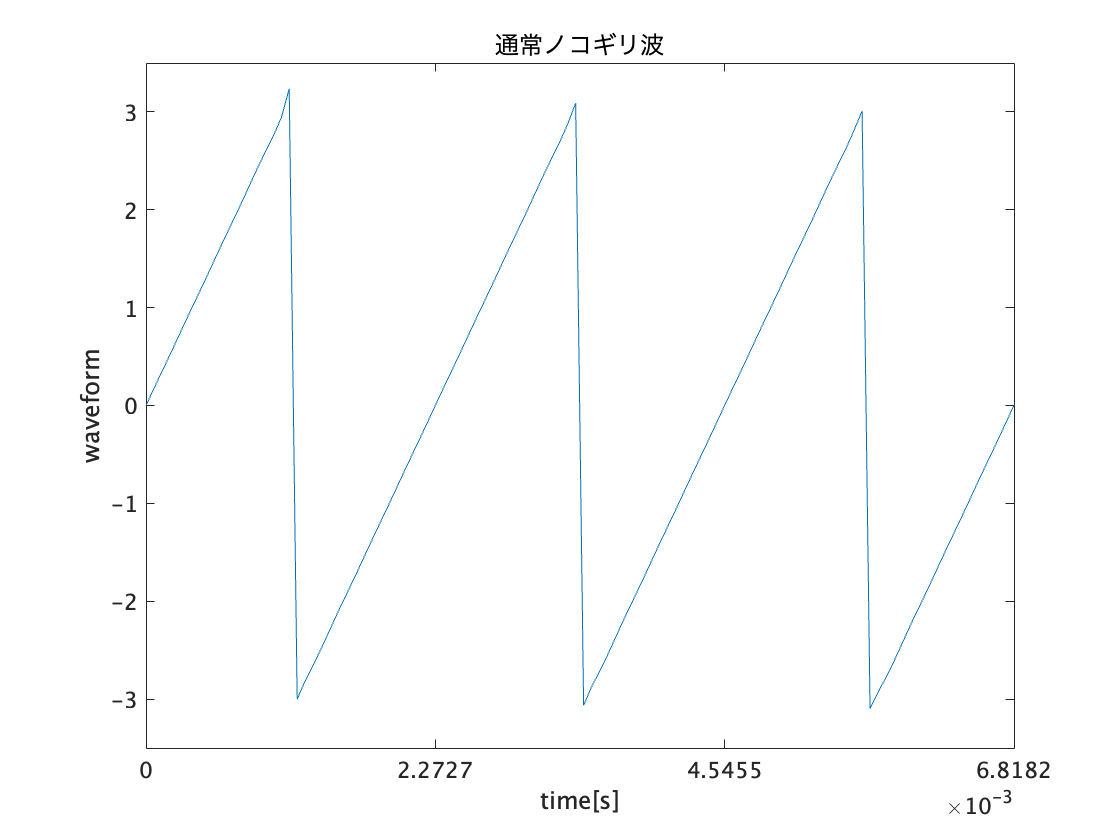
\includegraphics[keepaspectratio,height=0.5\textheight]{nokogiri.png}
    \end{figure}
\end{frame}
\subsection{フーリエ係数の分布}
\begin{frame}[t]{\showsec 周波数解析(フーリエ係数の分布)}
    \renewcommand{\arraystretch}{1.5}
    \begin{columns}
        \begin{column}[T]{0.44\textwidth}
            \begin{table}
                \begin{tabular}{r|cc}
                    \multicolumn{1}{c}{正弦波}   & 振幅                                                            & 周波数                                                             \\
                    \hline
                    \(2\sin(t)\)              & \tikz[remember picture,baseline=(A.base)]{\node(A){\(2\)}}    & \tikz[remember picture,baseline=(D.base)]{\node(D){\(1/2\pi\)}} \\
                    \(-\sin (2t)\)            & \(-1\)                                                        & \(1/\pi\)                                                       \\
                    \(\frac{2}{3}\sin (3t)\)  & \(2/3\)                                                       & \(3/2\pi\)                                                      \\
                    \(-\frac{1}{2}\sin (4t)\) & \tikz[remember picture,baseline=(C.base)]{\node(C){\(-1/2\)}} & \tikz[remember picture,baseline=(B.base)]{\node(B){\(2/\pi\)}}  \\
                    \multicolumn{3}{c}{{\LARGE\vdots}}
                \end{tabular}
            \end{table}
            \begin{tikzpicture}[remember picture,overlay]
                \node[inner sep=0.1mm,fit={(A)(B)(C)(D)},draw,rounded corners,draw=blue](warp){};
            \end{tikzpicture}
            \begin{align*}
                (-1)^{k-1}\dfrac{2}{k}\sin(kt) &  & (k\in\mathbb{N})
            \end{align*}
        \end{column}
        \begin{column}[T]{0.55\textwidth}
            \begin{figure}
                \caption{フーリエ係数の分布}
                \vspace{-1em}
                \begin{tikzpicture}[remember picture]
                    \node[left] at(0,0){O};
                    \draw[very thick,-Stealth](0,0)--(5,0)node[midway,fill=white]{\scriptsize 周波数};
                    \draw[very thick,-Stealth](0,-1.6)--(0,4.1)node[left]at($(0,0)!0.5!(0,4.1)$){\scriptsize \rotatebox{90}{振幅}};
                    \foreach \u \v in {0.4/3,0.8/-1.5,1.2/1,1.6/-0.75}
                    \draw[thick,blue](\u,0)--(\u,\v);
                    \foreach \u \v \z in {0.4/{\(1/2\pi\)}/below,0.8/{\(1/\pi\)}/above,1.2/{\(3/2\pi\)}/below,1.6/{\(2/\pi\)}/above}
                    \node[\z] at(\u,0){\tiny\v};
                    \coordinate (O) at (0,0);
                    \foreach \u \v \z \w in {0.4/3/a/{\(2\)},0.8/-1.5/b/{\(-1\)},1.2/1/c/{\(2/3\)},1.6/-0.75/d/{\(-1/2\)}} {
                    \coordinate (\z) at (\u,\v);
                    \draw[dotted,thin](\z)--(O |- \z)node[left]{\tiny\w};
                    }
                \end{tikzpicture}
                \begin{tikzpicture}[remember picture,overlay]
                    \draw[-latex,very thick,dashed]($(warp.south east)!0.5!(warp.south west)$)to[bend right=30]($(O)+(-0.5cm,0)$);
                \end{tikzpicture}
            \end{figure}
        \end{column}
    \end{columns}
\end{frame}
\subsection{高速フーリエ変換(\texttt{fft})}
\begin{frame}[t,containsverbatim]{\showsec 周波数分析(高速フーリエ変換 \texttt{fft})}
    サンプリング周波数\texttt{Fs}の信号\texttt{y}に対して高速フーリエ変換\texttt{fft}を行うだけでは周波数解析ができない!
    \begin{lstlisting}[language={Matlab},frame={lines},numbers={none},xleftmargin={0mm}]
fft_y = fft(y); % データ列yに対してfft を行う.
    \end{lstlisting}
    \begin{figure}
        \centering
        \begin{minipage}[t]{0.48\textwidth}
            \caption{\texttt{fft}を行った直後(\texttt{ftt\_y})}
            \label{fig:fft}
            \begin{tikzpicture}
                \draw[thick](0,0)--(0.9\textwidth,0)--(0.9\textwidth,0.5)--(0,0.5)--cycle;
                \node[below] at (0,0){\texttt{1}};
                \node[below] at (0.9\textwidth,0){\texttt{Fs}};
                \coordinate (C) at ($(0.9\textwidth,0)!0.5!(0,0)$);
                \draw[thick](C)--($(C)+(0,1.5mm)$);
                \coordinate (c) at ($(0.9\textwidth,0.5)!0.5!(0,0.5)$);
                \draw[thick](c)--($(c)+(0,-1.5mm)$);
                \node at($(C)!0.5!(0,5mm)$){\tiny 正のデータ};
                \node at($(c)!0.5!(0.9\textwidth,0mm)$){\tiny 負のデータ};
            \end{tikzpicture}
        \end{minipage}
        \begin{minipage}[t]{0.48\textwidth}
            \caption{理想的な状態}
            \label{fig:fftshift}
            \begin{tikzpicture}
                \draw[thick](0,0)--(0.9\textwidth,0)--(0.9\textwidth,0.5)--(0,0.5)--cycle;
                \node[below] at (0,0){\texttt{1}};
                \node[below] at (0.9\textwidth,0){\texttt{Fs}};
                \coordinate (C) at ($(0.9\textwidth,0)!0.5!(0,0)$);
                \draw[thick](C)--($(C)+(0,1.5mm)$);
                \coordinate (c) at ($(0.9\textwidth,0.5)!0.5!(0,0.5)$);
                \draw[thick](c)--($(c)+(0,-1.5mm)$);
                \node at($(C)!0.5!(0,5mm)$){\tiny 負のデータ};
                \node at($(c)!0.5!(0.9\textwidth,0mm)$){\tiny 正のデータ};
            \end{tikzpicture}
        \end{minipage}
    \end{figure}
    \begin{enumerate}
        \item 図\ref{fig:fft}から図\ref{fig:fftshift}の状態にするために\texttt{fftshift}関数を用いる.\\
              \begin{lstlisting}[language={Matlab},frame={lines},numbers={none},xleftmargin={0mm}]
fftshift_y = fftshift(fft_y);
            \end{lstlisting}
        \item 絶対値を取るために\texttt{abs}をとる.\\
              \begin{lstlisting}[language={Matlab},frame={lines},numbers={none},xleftmargin={0mm}]
fftshift_abs_y = abs(fftshift_y);
                        \end{lstlisting}
    \end{enumerate}
\end{frame}
\begin{frame}[t,containsverbatim]{\showsec 周波数分析(高速フーリエ変換 \texttt{fft})}

\end{frame}
\section{課題3}
\begin{frame}[t]{\showsec 課題3}
    \begin{exampleblock}{}
        \begin{enumerate}
            \item 課題2で録音した各音声を周波数解析し,スペクトル上でピークのある周波数およびその周波数のY軸の値を抽出しよう.
            \item 抽出した周波数,Y軸の値の順音を合成し,音の違いを聴き比べる.
        \end{enumerate}
    \end{exampleblock}
    \dotfill
    \begin{itemize}
        \item 0Hz - 10,000Hz 程度までの範囲で,ピークとなる周波数,及びそのピーク値を高い順から10個程度以上抽出する.\\
              (母音の識別に利用される主な周波数成分は4kHz以下)
        \item 周波数およびピーク値(Y軸の値)は厳密でなくて良い.
        \item \texttt{a},\texttt{i}の合成音の聞こえ方の違い,及び元の音声との違いについて考察する.
    \end{itemize}
\end{frame}
\subsection{サンプルコード}
\begin{frame}[t,containsverbatim]{\showsec 課題3(サンプルコード)}
    \begin{lstlisting}[language=Matlab]
clear all;

\end{lstlisting}
\end{frame}
\end{document}